\documentclass[11pt]{article}
\usepackage[utf8]{inputenc}
\usepackage{amsmath}
\usepackage{listings}
\usepackage{color}
\usepackage{graphicx}
\graphicspath{ {imagenes/} }

\lstset{
	language=C++,
    basicstyle=\ttfamily,
    keywordstyle=\color{blue}\ttfamily,
    stringstyle=\color{red}\ttfamily,
    commentstyle=\color{green}\ttfamily,
    morecomment=[l][\color{magenta}]{\#}
}

\title{\textbf{Laboratorio Tarea B Implementación}}
\author{Paolo Montero\\
		Obdulio Varela\\
		Indio Arispe}
\date{}
\begin{document}

\maketitle
\newpage
\tableofcontents
\newpage
\section{Formalización}

\begin{itemize}
\item  Forma de Solución
\end{itemize}

$<x_0, x_1,..., x_{n-1}>$ tupla de largo \textbf{n}, donde \textbf{n} es la cantidad de charlas.

\begin{itemize}
\item  Restricciones explícitas
\end{itemize}

$-1 \leq x_i \leq m-1$ con $0 \leq i \leq n-1$, \newline
donde \textbf{n} es la cantidad de charlas, \textbf{m} es la cantidad de salas

\begin{itemize}
\item  Restricciones implícitas
\end{itemize}

Dos charlas pertenecen  la misma sala si son compatibles.

\[
    compatibles(i,j)= 
\begin{cases}
    true,& \text{if } charlas[i].fin \leq charlas[j].inicio\\ \lor \  charlas[j].fin \leq charlas[i].inicio\\
    false,              & \text{otro caso}
\end{cases}
\]


Una charla es asignada a una sala solo si la sala tiene disponibilidad horaria para abarcar la charla.

\[
    disponible(x_i,i)= 
\begin{cases}
    true,& \text{if } charlas[i].fin \leq salas[x_i].fin\\ \land \  charlas[i].inicio \geq salas[x_i].inicio\\
    false,              & \text{otro caso}
\end{cases}
\]

\begin{itemize}
\item  Función objetivo
\end{itemize}

Devuelve aquella solución que asegura la máxima asistencia.


\[ T = \{ t=<x_0, x_1, ..., x_{n-1}> \  t \  es \  solucion\}\]

\[ f(t)=max_{t \in T} \{ cantAsistentes(t) \}\]

\[ cantAsistentes(t) = \sum\limits_{i=0}^{i=n-1} \delta(x_i) charlas[i].asistentes \]

\[ \delta(x_i) = 
\begin{cases}
    0,& \text{if } x_i = -1 \\
    1,              & \text{otro caso}
\end{cases}
\]


\section{Recorrida Backtracking}
\subsection{Comentarios sobre recorridas}
\begin{itemize}
\item  \textbf{Caso tres charlas dos salas}
\end{itemize}

Una recorrida que nos sirve es esta

\begin{center}
  \makebox[\textwidth]{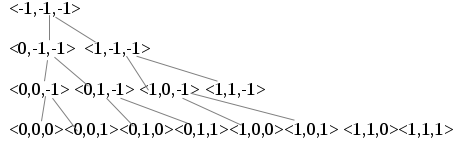
\includegraphics{recorrida01}}
\end{center}

Pero dadas las restricciones de que una sala cualquiera puede estar o no  debemos hacer recorridas anulando salas.

Por ejemplo un recorrido que no considere la primera sala.

\begin{center}
  \makebox[\textwidth]{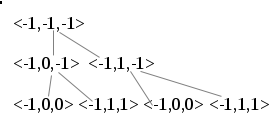
\includegraphics{recorrida02}}
\end{center}

Estas soluciones no son contempladas en la primera recorrida, por lo que para llegar a estas hay que meter una recorrida imponiendo que la primera charla no sea considerada.

También puede ser de interés considerar las combinaciones de la primera y tercera charla y ver que soluciones salen sin tener en cuenta a la segunda.

\begin{center}
  \makebox[\textwidth]{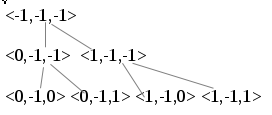
\includegraphics{recorrida03}}
\end{center}

El recorrido debería considerar estas soluciones también. \newpage

\subsection{Propuesta de algoritmo}

El algoritmo adjunto trata de cubrir el arbol de soluciones teniendo en cuenta las consideraciones de la sección 2.1 de la siguiente manera.


\begin{lstlisting}
//Declaracion de funcion
void backtracking(charla* charlas, int n, sala* salas, int m, 
int *solucion, int i, int *tupla, int parche);
//Extracto del codigo sucesivas llamadas a BackTracking
	printf("BackTrackin!! \n");
	//Se trata de cubrir los agujeros con un parche
	//que lo que hace es para cada pasada va silenciando
	//a las salas.
	for(int i=0; i < n; i++)
	{
		for(int j=0; j < n; j++)
		{
			tupla[j]=-1;

		}

 		for(int k=i-1; k < n; k++){
 
			backtracking(charlas, n, salas, m,
			 solucion, i, tupla, k);
		}
	}
	
\end{lstlisting}
\newpage
\begin{lstlisting}
void backtracking(charla* charlas, int n, sala* salas, int m, 
int *solucion, int i, int *tupla, int parche)
{
//Recorrida correcta de cada componente
//probando con diferentes salas para cada charla
//obviando a las charlas silenciadas por el parche

		for(int xi=0; xi < m; xi++)
			{
					if(i==parche)
						i=i+1;
					if(i<n){
						tupla[i]=xi;
						backtracking(charlas, 
						n, salas, m, 
						solucion, i + 1, 
						tupla, parche);
						if(tupla[i]=m)
							tupla[i]=-1;							
					}
		}
}

\end{lstlisting}

\end{document}
